\section{Introduction}

\begin{frame}
\frametitle{Introduction}
\framesubtitle{What is issue tracking?}

\begin{block}{It means to keep a registry of problems encountered}
\begin{itemize}
\item Publish issues for later reference
\item Assign issues to a specific developers
\item Organize issues based on category and priority
\end{itemize}
\end{block}

\end{frame}

\begin{frame}
\frametitle{Introduction}
\framesubtitle{Why issue tracking?}

\begin{block}{Problems must be remembered or reminded}
\begin{itemize}
\item Even if for yourself only, use issue tracking to take notes of problems to deal with
\item When issues surface on other's code, you need to make people know
\end{itemize}
\end{block}

\end{frame}

\begin{frame}
\frametitle{Introduction}
\framesubtitle{Issue tracking is not only about problems}

\begin{block}{You can also issue proposals or enhancements}
\begin{itemize}
\item New features can be proposed and discussed with other developers
\item Existing features can be enhanced to address a new requirement
\end{itemize}
\end{block}

\end{frame}

\section{BitBucket}

\begin{frame}
\frametitle{Bitbucket}
\framesubtitle{Why BitBucket?}

\begin{block}{BitBucket is not the only player out there}
\begin{itemize}
\item It is just a convenient website with adequate tools. It also hosts our remote Git repositories.
\end{itemize}
Issue tracking, with small changes, applies to Google Code rather than GitHub rather than JIRA or others. 
\end{block}

\end{frame}

\begin{frame}
\frametitle{BitBucket}
\framesubtitle{Registration}

\medskip

You can register at \url{https://bitbucket.org/account/signup/}

\begin{figure}
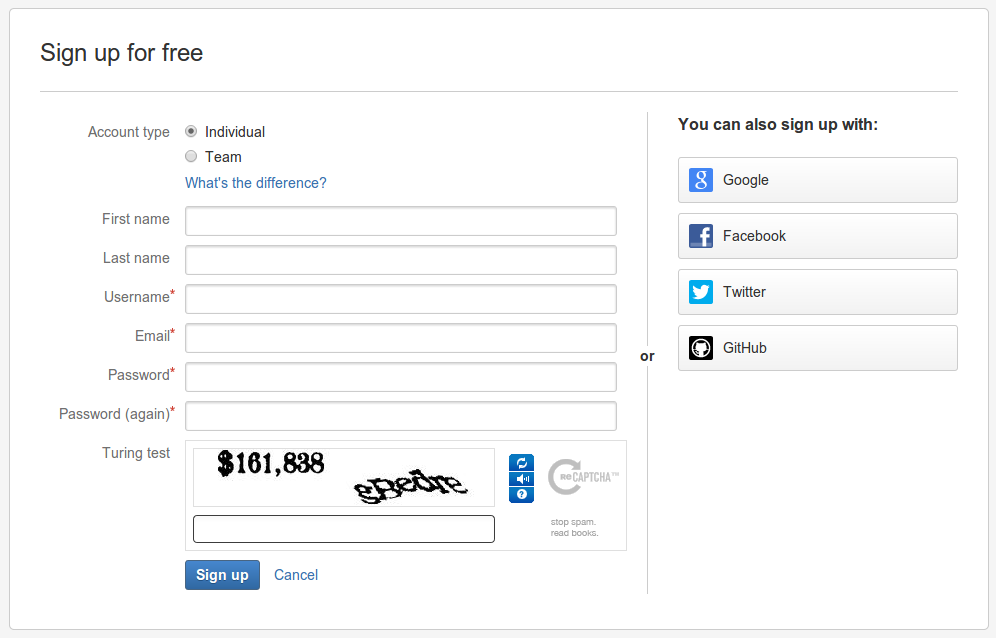
\includegraphics[width=1.0\textwidth]{lecture04/img/createnewaccount.png}
\end{figure}

\end{frame}

\begin{frame}
\frametitle{BitBucket}
\framesubtitle{Registration}

\begin{block}{Instructions}
\begin{itemize}
\item Create an individual account, preferably your surname prefixed by the first letter of your name, like \texttt{lgeretti}
\item Use your \texttt{@spes.uniud.it} email account, since the account will be recognized as Academic
\end{itemize}
\end{block}
\begin{block}{Features}
\begin{enumerate}
\item unlimited public repositories;
\item unlimited private repositories;
\item (if you have an Academic account) unlimited collaborators;
\item issue tracking
\item Forking
\item Wiki
\end{enumerate}
\end{block}

\end{frame}

\begin{frame}
\frametitle{BitBucket}
\framesubtitle{Your first repository}

\medskip 

You can create a new empty remote repository at \url{https://bitbucket.org/repo/create}

\begin{figure}
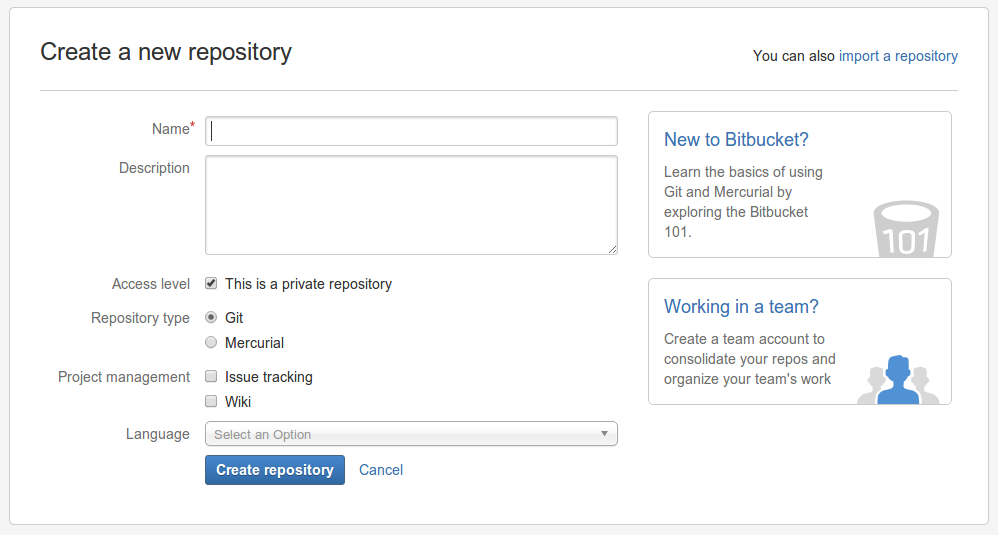
\includegraphics[width=1.0\textwidth]{lecture04/img/createnewrepo.png}
\end{figure}

\end{frame}

\begin{frame}
\frametitle{BitBucket}
\framesubtitle{Your first repository}

\begin{block}{Instructions}
\begin{itemize}
\item Choose a name, e.g., \texttt{testing}, keep Git as repo type and add Issue Tracking
\item Keep it private (unless you invite users, they cannot see it)
\item You can add a description and choose a language type for easy reference
\item After creating it, the Get Started page gives you suggestions on how to start
\end{itemize}
\end{block}

\end{frame}

\begin{frame}
\frametitle{BitBucket}
\framesubtitle{Let us play a little with Git}

\begin{block}{You can clone your (empty) remote repo}
\begin{itemize}
\item Find the command by clicking the \texttt{Clone} button
\item You can choose \texttt{HTTPS} or \texttt{SSH} R/W access
\end{itemize}
\end{block}

\begin{block}{(optional) Set a key for SSH}
HTTPS always asks for a password. Using SSH with a key avoids asking for a password each time. 
\begin{itemize}
\item Go to your \texttt{Manage Account} page (upper right)
\item Choose \texttt{SSH Keys} to add access with asymmetric keys
\item Follow instructions to create a public+private key on your machine and to import the public key into BitBucket
\item Now all access from a machine where the private key is present will be secure and passless
\end{itemize}
\end{block}

\end{frame}

\section{Issue tracking}

\begin{frame}
\frametitle{BitBucket}
\framesubtitle{Your first issue}

\begin{figure}
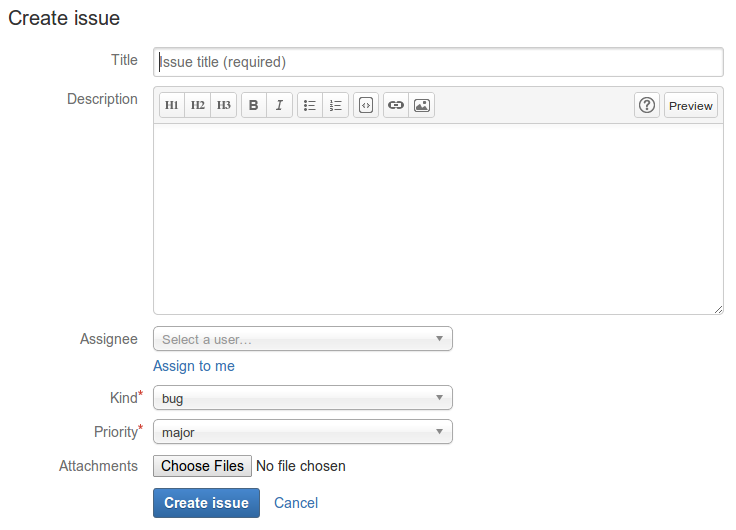
\includegraphics[width=1.0\textwidth]{lecture04/img/createnewissue.png}
\end{figure}

\end{frame}

\begin{frame}
\frametitle{BitBucket}
\framesubtitle{Title and description}

You can create a new issue for a repository under \texttt{Issues}.

\bigskip

\begin{block}{You need a title and a description}
\begin{itemize}
\item The title should just summarize the issue at hand
\item The description provides more detail to address the issue
\item You can format the description as a Wiki page, even adding images
\end{itemize}
\end{block}

\end{frame}

\begin{frame}
\frametitle{BitBucket}
\framesubtitle{Kind and priority}

\begin{block}{The kind is a category}
\begin{itemize}
\item Bug: notify that something does not work as expected
\item Enhancement: put a request for an improvement on something existing
\item Proposal: put a request for an additional feature
\item Task: some activity not strictly related to code writing, like reviewing code
\end{itemize}
\end{block}

\begin{block}{The priority signals importance}
You should use \texttt{blocker} only when it stops you from further work
\end{block}

\end{frame}

\begin{frame}
\frametitle{BitBucket}
\framesubtitle{Assignee and attachments}

\begin{block}{The assignee is a proposal}
You can assign someone to the issue, if you are certain: he will be notified.
\end{block}

\begin{block}{Attachments complement the issue}
\begin{itemize}
\item Bug reports or logs
\item Patch files
\item Images or documents for a proposal
\end{itemize}
\end{block}

\end{frame}

\begin{frame}
\frametitle{BitBucket}
\framesubtitle{Issue listing}

Issues can be filtered by kind, priority, etc. Each one can be selected for additional info.

\bigskip

\begin{figure}
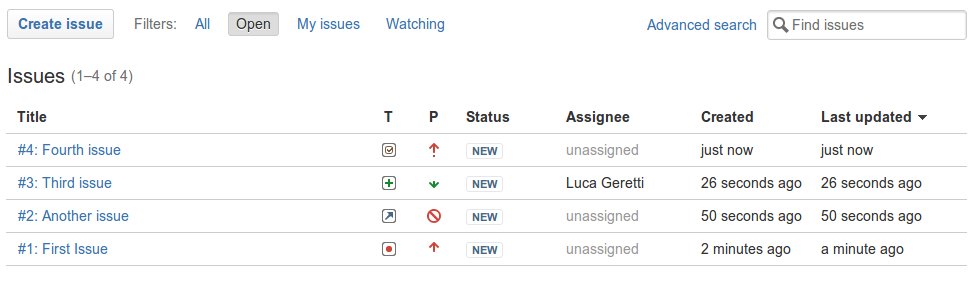
\includegraphics[width=1.0\textwidth]{lecture04/img/issueselection.png}
\end{figure}

\end{frame}

\begin{frame}
\frametitle{BitBucket}
\framesubtitle{Issue summary}

\begin{block}{Issues are not written in stone}
\begin{itemize}
\item Issues can be simply {\em resolved} when addressed, but usually they evolve during development
\item They can be commented
\item They can be edited
\item They can be removed without resolution
\end{itemize}
\end{block}

\begin{figure}
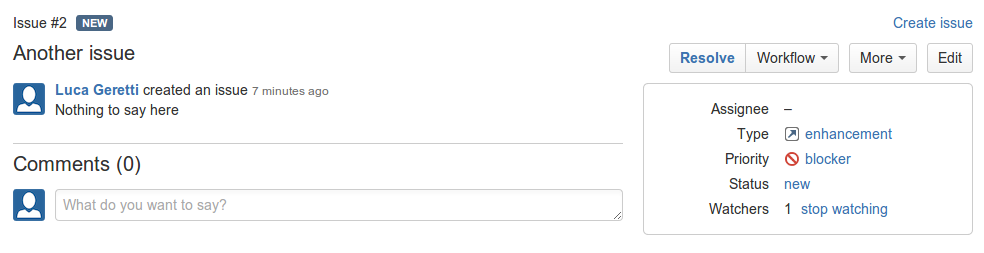
\includegraphics[width=1.0\textwidth]{lecture04/img/issuecontrol.png}
\end{figure}

\end{frame}

\begin{frame}
\frametitle{BitBucket}
\framesubtitle{Issue status}

\begin{block}{Under \texttt{Workflow}, issue status can be changed}
\begin{itemize}
\item New: has been created, but no one has started work on it
\item Open: resolution of the issue has started
\item On hold: has been opened, but work on it has been paused
\item Resolved: has now been resolved, i.e., it is closed (same as choosing the \texttt{Resolve} button)
\item Duplicate: useless issue, as it is the same as another one
\item Invalid: it does not apply for some reason
\item Wontfix: the bug is acknowledged, but it will not be addressed for some reason
\end{itemize}
A comment is usually welcome, to explain state changes.
\end{block}

\end{frame}